\documentclass[12pt, twoside]{article}
% \documentclass[12pt, twoside]{article}
\usepackage[letterpaper, margin=1in, headsep=0.2in]{geometry}
\setlength{\headheight}{0.6in}
%\usepackage[english]{babel}
\usepackage[utf8]{inputenc}
\usepackage{microtype}
\usepackage{amsmath}
\usepackage{amssymb}
%\usepackage{amsfonts}
\usepackage[nomessages]{fp} %\FPeval{\var-name}{2*sin(pi/6)}
\usepackage{siunitx} %units in math. eg 20\milli\meter
\usepackage{yhmath} % for arcs, overparenth command
\usepackage{tikz} %graphics
\usetikzlibrary{quotes, angles, arrows, arrows.meta}
\usepackage{graphicx} %consider setting \graphicspath{{images/}}
\usepackage{parskip} %no paragraph indent
\usepackage{enumitem}
\usepackage{multicol}
\usepackage{venndiagram}

\usepackage{fancyhdr}
\pagestyle{fancy}
\fancyhf{}
\renewcommand{\headrulewidth}{0pt} % disable the underline of the header
\raggedbottom
\hfuzz=2mm %suppresses overfull box warnings

\usepackage{hyperref}

\fancyhead[LE]{\thepage}
\fancyhead[RO]{\thepage \\ Name: \hspace{4cm} \,\\}
\fancyhead[LO]{BECA / Dr. Huson / Geometry\\*  Unit 4: Trigonometry \\* 31 January 2025}

\begin{document}

\subsubsection*{10.18 Unit Test: Trigonometry \hfill HSG.SRT.C.8}
\begin{enumerate}
\item As shown, right $\triangle ABC$ has $AC=5, BC=12, AB=13$, m$\angle C=90^\circ$. \\[0.25cm] 
Express each trigonometric ratio as a fraction.
  \begin{multicols}{2}
    \begin{enumerate}
      \item $\sin A =$
      \item $\cos A =$
      \item $\tan A =$ 
      \item Find the angle measure of $\angle A$ rounded to the \emph{nearest whole degree}. \vspace{1cm}
    \end{enumerate}
    \begin{center}
      \begin{tikzpicture}[scale=0.4]
        \draw [thick](0,0) node[below]{$A$}--
        (4,0) node[below]{$C$}--
        (4,9) node[above right]{$B$}--cycle;
        \node at (2,-1){$5$};
        \node at (4,4)[right]{$12$};
        \node at (1,4.5){$13$};
        \draw (4,0)++(-0.6,0)--++(0,0.6)--+(0.6,0);
        \draw (0.75,0) arc [start angle=0, end angle=63, radius=0.75];
      \end{tikzpicture}
    \end{center}
  \end{multicols} \vspace{0.25cm}

\item Isosceles right $\triangle ABC$ is shown with legs $AC=BC=1$ as marked.\vspace{0.25cm}
  \begin{multicols}{2}
    \begin{enumerate}
      \item Write down $\theta$.
      \item Find the length of hypotenuse $AB$ as an exact expression.\vspace{2cm}
    \end{enumerate}
    \begin{flushright}
      \begin{tikzpicture}[scale=0.7]
        \draw [thick](0,0)node[below]{$A$}--
        (5,0)node[below]{$C$}--
        (5,5)node[above right]{$B$}--cycle;
        \draw (5,0)++(-0.6,0)--++(0,0.6)--+(0.6,0);
        \node at (2.5,0)[below]{$1$};
        \node at (5,2.5)[right]{$1$};
        \draw [thick, -] (1,0) arc [start angle=0, end angle=45, radius=1];
        \node at (1.2,0.1)[above]{$\theta$};
      \end{tikzpicture}
    \end{flushright}
  \end{multicols}

\newpage
\item At an angle of elevation of $15^\circ$, the top of a structure $B$ is visible from point $A$ on the ground 50 meters away, as shown below.

Find the height $h$ of the structure to the \emph{nearest tenth of a meter}. \hfill (not to scale)
  \begin{flushright}
    \begin{tikzpicture}[scale=0.3]
      %\draw [-, thick] (0,0)--(35:23);
      \draw [-, thick] (-4,0)--
      (0,0)--
        (17,0)--
        (22,0)--
        (22,10)--(17,10)--(17,0);
      \draw [fill] (0,0) circle [radius=0.1] node[above left]{$A$};
      \draw [fill] (17,10) circle [radius=0.1] node[above right]{$B$};
      \draw [dashed] (0,0)--(17,10);
      \node at (3.8, 0)[above]{$15^\circ$};
      \node at (11, 0)[below]{50 m};
      \node at (17, 5)[right]{$h$};
    \end{tikzpicture}
    \end{flushright} \vspace{3cm}


\item A 15-foot ladder leans against a building and reaches a window 12 feet above ground. What is the measure of the angle, to the \emph{nearest degree}, that the ladder forms with the ground?

\item A man was parasailing above a lake at an angle of elevation of $32^\circ$ from a boat, as modeled in the diagram below.
  \begin{center}
    \includegraphics[width=9cm]{../graphics/parasail.png}
  \end{center}
If 129.5 meters of cable connected the boat to the parasail, approximately how many meters above the lake was the man? (to the \emph{nearest tenth of a meter})

\newpage
\item Regents problem \\
\includegraphics[width=16cm]{../graphics/marina.png}


\end{enumerate}
\end{document}
  